\chapter{Literature Review}
\section{Associative Memory}
Associative memory also known as content addressable memory is a type of memory
which is specially optimized for access to memory locations without using the
memory address of the location that needs to be accessed. Its electronic
circuit will have extra connections which enable it to parallelly search
through the contents in a single clock pulse. It is widely used in applications
like database management systems which require searching through the data as
fast as possible figure \ref{associative_circuit} shows one such circuit.
\begin{figure}[h!]
    \centering
    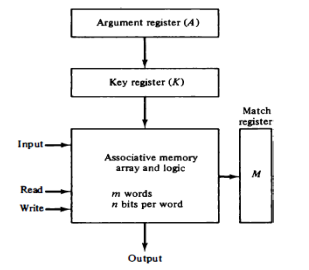
\includegraphics[width=0.7\linewidth]{associative}
    \caption{Associative memory circuit}
    \label{associative_circuit}
\end{figure}
% Associative memory systems are a type of artificial intelligence technology
% that is used for storing and retrieving information based on patterns or
% associations. They are commonly used in applications such as pattern
% recognition, data storage, and information retrieval.
\section{Neural associative memory}
Neural associative memory is also known as the associative network, which works
based on pattern association. It can store different patterns and produce the
output which closely matches the already given patterns. They are implemented
using the artificial neural network, which tries to mimic the working of the
brain. They are commonly used in applications like pattern recognition, data
storage and information retrieval. There are two types of associative networks
\begin{description}
    \item[Auto associative memory]A single layer \nn in which the number of training
    vectors and the number of output vectors are the same. The weights are
    determined by the stored patterns
    \item[Hetero associative memory]A single layer \nn in which the number of input
    training vectors and output are different. Weights are determined by the
    pattern stored in the network. It is static in nature and hence there would be
    no linear or delay operations
\end{description}

\subsection{Hopfield model}
The Hopfield model \cite{hopfield} is a type of \rnn. The model is designed to
mimic the behaviour of neurons in the brain. It is a type of associative memory
system and hence it can store and recall information based on the relationship
between the data stored. It has application including pattern recognition,
optimization, and error correction.

It is a fully connected \nn and weights between connections determine the
strength of the connections. When the network is supplied with an input these
weights are updated sequentially until the network reaches a stable state, at
which the output is determined. By adjusting the weights in a specific way, the
the network is able to recall the information as a set of stable states

The main drawbacks of the model are that it may not converge to correct output
state when it is supplied with a pattern which is only partially similar to the
stored patterns or when it is not trained on sufficiently distinct data and is
that it is not well suited for dealing with a large amount of data because the
number of connections increased when the number of nodes increased. It makes it
difficult to train on large datasets.

\section{\Snn}
Spiking neural networks are a type of neural network that models the behaviour
of biological neurons by using spikes or pulses to encode and transmit
information. They are a relatively new type of neural network that has the
potential to improve the performance and efficiency of artificial intelligence
systems. The use of spiking neural networks for building associative memory
systems is a relatively new area of research that has only recently started to
gain attention.
\subsection{Spike time dependent plasticity}
Spike time dependent plasticity (STDP) is an unsupervised learning rule based
on the functioning of neurons in the brain. In the process strength of
connection between neurons change based on the relative timing of spikes or
impulses

The basic idea behind STDP is that if two $N_{pre}$ and $N_{suc}$ neurons are
connected and their spike time are $t_1$ and $t_2$ respectively according to
STDP
\begin{itemize}
    \item[]Weight of connection from $N_{pre}$ to $N_{suc}$ should  increase, if $t_1>t_2$

    \item[]Weight of connection from $N_{pre}$ to $N_{suc}$ should  decrease, if $t_1<t_2$
    \item[]Weight of connection from $N_{pre}$ to $N_{suc}$ should  remain same, if $t_1=t_2$
\end{itemize}
\subsection{SpikeProp}

% Associative memory systems: This would involve reviewing the existing research
% on different types of associative memory systems, such as Hopfield networks,
% boltzmann machines, and autoencoders. We would also review the key algorithms
% and techniques used for training and evaluating associative memory systems.

% Spiking neural networks: This would involve reviewing the existing research on
% spiking neural networks, including their principles, architectures, and
% applications. We would also review the key algorithms and techniques used for
% training and evaluating spiking neural networks.

% Combining associative memory and spiking neural networks: This would involve
% reviewing the existing research on approaches for combining the capabilities of
% associative memory systems and spiking neural networks. We would also review
% the key challenges and limitations of these approaches, and the current state
% of the art in this area.

% Technical\cite{base} writing is writing or drafting technical communication
% used in technical and occupational fields\cite{india}, such as computer
% hardware and software\cite{rpi}, engineering, chemistry, aeronautics, robotics,
% finance\cite{japan}, medical, consumer electronics, biotechnology, and
% forestry. Technical writing encompasses the largest sub-field in technical
% communication. See figure \ref{net2} that shows the autonomous systems in
% Internet.

% \begin{figure}[h!]
% 	\centering
% 	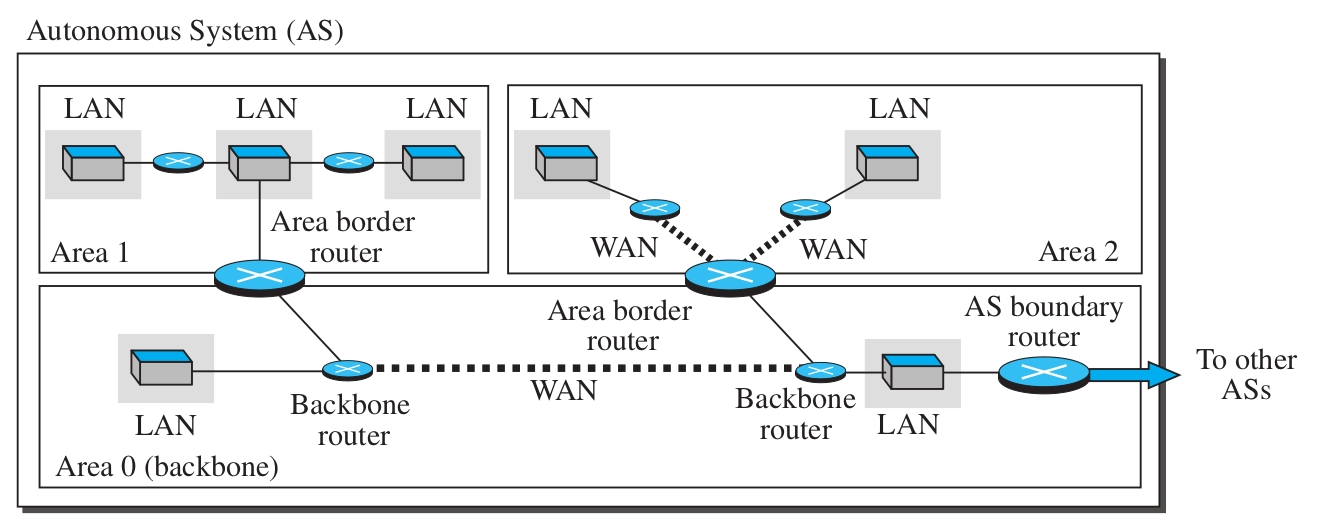
\includegraphics[width=0.9\linewidth]{ospf}
% 	\caption{Autonomous System Hierarchy}
% 	\label{net2}
% \end{figure}

% \section{section1}
% \lipsum[2] % Please comment this line and type in the introduction chapter

% \subsection{title 2}
% \lipsum[3] % Please comment this line and type in the introduction chapter

% \noindent The system is described by the equation \ref{sys_eq1} below. Here y is the ordinate and x is the abscissa , m is the slope and c a constant.

% \begin{equation} \label{sys_eq1}
% 	y = mx + c
% \end{equation}
% \noindent Page centered and unnumbered multiple equations. The * symbol supresses equation numbering.
% % Page centered and unnumbered equations
% \begin{align*}
% 	2x - 5y & =  8   \\
% 	3x + 9y & =  -12
% \end{align*}

% \noindent Side by side figures can be created using this environment. See fig \ref{wave} below.
% \begin{figure}[h!]
% 	\centering
% 	\begin{subfigure}[b]{0.4\textwidth}
% 		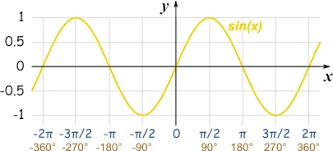
\includegraphics[width=\textwidth]{sinewave}
% 		\caption{Sine Wave}
% 		\label{fig:1}
% 	\end{subfigure}
% 	\hspace{20mm}
% 	\begin{subfigure}[b]{0.4\textwidth}
% 		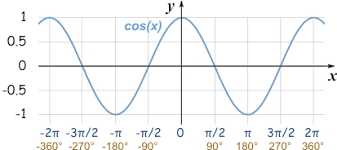
\includegraphics[width=\linewidth]{cosine}
% 		\caption{Cosine Wave}
% 		\label{fig:2}
% 	\end{subfigure}
% 	\caption{The Sine and Cosine waves}
% 	\label{wave}
% \end{figure}